%!TEX root = ../main.tex

\chapter{Germanium detector models}%
\label{apdx:gedetav}

As a result of the presence of the \nplus\ contact on the outer surface of the germanium
detectors, the charge-collection efficiency (CCE) differs from unity in the region close
to the contact. As a matter of fact, lithium impurities diffused inside the crystal during
the diode fabrication process act as recombination centers for charge carriers, and the
CCE curve strongly depends on the lithium concentration profile. Such a situation
typically leads to events depositing energy in this region being characterized by a lower
reconstructed energy, depending on the local CCE. The reader is referred
to~\cite{Lehnert2016} for an extensive discussion of the charge-collection mechanism in
germanium detectors and CCE models.

\begin{figure}
  \centering
  \includegraphics{setup/gedet-av/tl-model.pdf}
  \caption{%
    Germanium detector active volume model. The charge-collection efficiency is zero by
    definition at the outer surface and remains such through all the `dead layer'. The
    detector is partially active in the `transition layer' region, where the CCE gradually
    increases until reaching its maximal value in the fully active volume.
  }\label{fig:gedetav:tl-model}
\end{figure}

\blocktitle{fully \\ active \\ volume}
The full charge-collection depth (FCCD), defined as the depth at which the CCE reaches
unity, has been estimated for each germanium detector deployed in \gerda\ during dedicated
characterization campaigns. In these measurements, a radioactive source (e.g.~\Am, \Ba,
\Co) is positioned close to the detector surface to sample its energy spectrum. A matching
between data and Monte Carlo simulations is then performed to find the FCCD value that
best describes data. The recommended FCCD values obtained from this characterization data
are reported in \cref{tab:gedetav:official}. The \scoax\ values are extracted from \Co\
data as documented in~\cite{Heider2009}, while the \bege\ values are obtained combining
\Am\ and \Ba\ data~\cite{Agostini2019}. \icoax\ values are extracted from \Am\
measurements. The \bege\ detectors have been stored at room temperature in the time
interval between their characterization to the deployment in liquid argon, and must be
therefore corrected for the dead-layer growing effect. The growth speed at room
temperature has never been determined rigorously, and the best available estimate is of
about $\sim{}0.1$~mm/yr, with a standard deviation of 0.04~mm/yr (\cite{Agostini2019} and
references therein). The correction is therefore applied considering the exact time spent
by each detector at room temperature together with an additional systematic uncertainty of
50\%.
\begin{table}
  \centering
  \caption{%
    Recommended full charge-collection depth (FCCD) and dead layer fraction (DLF) values
    for each detector deployed in \gerdatwo, calculated from detector characterization
    data. The \bege\ FCCD values are obtained combining \Am\ and \Ba\
    data~\cite{Agostini2019} while \scoax\ values are extracted from \Co\
    data~\cite{Heider2009}. The \icoax\ values are obtained from \Am\ data. The \bege\
    FCCDs are corrected for the dead-layer growing effect at room temperature experienced
    before installment in \gerda~\cite{Agostini2019}. The uncertainties are split into
    correlated and uncorrelated contributions. The DLF values have been estimated
    in~\cite{Lehnert2016} and do not include any growing effect at room temperature.
    \fillme{fill table}
  }\label{tab:gedetav:official}
  \newcommand{\mes}[3]{\measurement{#1}{#2}{#3}}
\newcommand{\mep}[5]{${#1}\substack{+#2\,+#3 \\ -#4\,-#5}$}

\begin{tabular}{rcc}
  \toprule
  Detector & FCCD (mm)                          & DLF                    \\
  \midrule
  \ANG{1}  & \mep{0.00}{0.00}{0.00}{0.00}{0.00} & --                     \\
  \ANG{2}  & \mep{0.00}{0.00}{0.00}{0.00}{0.00} & --                     \\
  \ANG{3}  & \mep{0.00}{0.00}{0.00}{0.00}{0.00} & --                     \\
  \ANG{4}  & \mep{0.00}{0.00}{0.00}{0.00}{0.00} & --                     \\
  \ANG{5}  & \mep{0.00}{0.00}{0.00}{0.00}{0.00} & --                     \\
  \RG{1}   & \mep{0.00}{0.00}{0.00}{0.00}{0.00} & --                     \\
  \RG{2}   & \mep{0.00}{0.00}{0.00}{0.00}{0.00} & --                     \\
  \midrule
  \GD{00A} & \mep{0.91}{0.15}{0.03}{0.14}{0.05} & \mes{0.17}{0.05}{0.04} \\
  \GD{00B} & \mep{0.00}{0.00}{0.00}{0.00}{0.00} & \mes{0.00}{0.00}{0.00} \\
  \GD{00C} & \mep{0.00}{0.00}{0.00}{0.00}{0.00} & \mes{0.00}{0.00}{0.00} \\
  \GD{00D} & \mep{0.00}{0.00}{0.00}{0.00}{0.00} & \mes{0.00}{0.00}{0.00} \\
  \GD{02A} & \mep{0.00}{0.00}{0.00}{0.00}{0.00} & \mes{0.00}{0.00}{0.00} \\
  \GD{02B} & \mep{0.00}{0.00}{0.00}{0.00}{0.00} & \mes{0.00}{0.00}{0.00} \\
  \GD{02C} & \mep{0.00}{0.00}{0.00}{0.00}{0.00} & \mes{0.00}{0.00}{0.00} \\
  \GD{02D} & \mep{0.00}{0.00}{0.00}{0.00}{0.00} & \mes{0.00}{0.00}{0.00} \\
  \GD{32A} & \mep{0.00}{0.00}{0.00}{0.00}{0.00} & \mes{0.00}{0.00}{0.00} \\
  \GD{32B} & \mep{0.00}{0.00}{0.00}{0.00}{0.00} & \mes{0.00}{0.00}{0.00} \\
  \GD{32C} & \mep{0.00}{0.00}{0.00}{0.00}{0.00} & \mes{0.00}{0.00}{0.00} \\
  \GD{32D} & \mep{0.00}{0.00}{0.00}{0.00}{0.00} & \mes{0.00}{0.00}{0.00} \\
  \GD{35A} & \mep{0.00}{0.00}{0.00}{0.00}{0.00} & \mes{0.00}{0.00}{0.00} \\
  \GD{35B} & \mep{0.00}{0.00}{0.00}{0.00}{0.00} & \mes{0.00}{0.00}{0.00} \\
  \bottomrule
\end{tabular}
\quad
\begin{tabular}{rcc}
  \toprule
  Detector & FCCD (\mum)                        & DLF                    \\
  \midrule
  \GD{35C} & \mep{0.00}{0.00}{0.00}{0.00}{0.00} & \mes{0.00}{0.00}{0.00} \\
  \GD{61A} & \mep{0.00}{0.00}{0.00}{0.00}{0.00} & \mes{0.00}{0.00}{0.00} \\
  \GD{61B} & \mep{0.00}{0.00}{0.00}{0.00}{0.00} & \mes{0.00}{0.00}{0.00} \\
  \GD{61C} & \mep{0.00}{0.00}{0.00}{0.00}{0.00} & \mes{0.00}{0.00}{0.00} \\
  \GD{76B} & \mep{0.00}{0.00}{0.00}{0.00}{0.00} & \mes{0.00}{0.00}{0.00} \\
  \GD{76C} & \mep{0.00}{0.00}{0.00}{0.00}{0.00} & \mes{0.00}{0.00}{0.00} \\
  \GD{79B} & \mep{0.00}{0.00}{0.00}{0.00}{0.00} & \mes{0.00}{0.00}{0.00} \\
  \GD{79C} & \mep{0.00}{0.00}{0.00}{0.00}{0.00} & \mes{0.00}{0.00}{0.00} \\
  \GD{89A} & \mep{0.00}{0.00}{0.00}{0.00}{0.00} & \mes{0.00}{0.00}{0.00} \\
  \GD{89B} & \mep{0.00}{0.00}{0.00}{0.00}{0.00} & \mes{0.00}{0.00}{0.00} \\
  \GD{89C} & \mep{0.00}{0.00}{0.00}{0.00}{0.00} & \mes{0.00}{0.00}{0.00} \\
  \GD{89D} & \mep{0.00}{0.00}{0.00}{0.00}{0.00} & \mes{0.00}{0.00}{0.00} \\
  \GD{91A} & \mep{0.00}{0.00}{0.00}{0.00}{0.00} & \mes{0.00}{0.00}{0.00} \\
  \GD{91B} & \mep{0.00}{0.00}{0.00}{0.00}{0.00} & \mes{0.00}{0.00}{0.00} \\
  \GD{91C} & \mep{0.00}{0.00}{0.00}{0.00}{0.00} & \mes{0.00}{0.00}{0.00} \\
  \GD{91D} & \mep{0.99}{0.16}{0.03}{0.16}{0.06} & \mes{0.36}{0.04}{0.03} \\
  \midrule
  \IC{48A} & \mep{0.00}{0.00}{0.00}{0.00}{0.00} & --                     \\
  \IC{48B} & \mep{0.00}{0.00}{0.00}{0.00}{0.00} & --                     \\
  \IC{50A} & \mep{0.00}{0.00}{0.00}{0.00}{0.00} & --                     \\
  \IC{50B} & \mep{0.00}{0.00}{0.00}{0.00}{0.00} & --                     \\
  \IC{74A} & \mep{0.00}{0.00}{0.00}{0.00}{0.00} & --                     \\
  \bottomrule
\end{tabular}

\end{table}

\blocktitle{transition \\ layer}
The region enclosed by the detector surface and the FCCD is, of course, not completely
dead, and regions with reduced CCE are expected. The CCE curve in this region strongly
depends on the lithium concentration profile, which is in turn strongly dependent on the
diode fabrication process (initial lithium concentration at the surface, thermal annealing
cycles etc.) and is \emph{a priori} different for each detector. As a consequence, the
transition region must be characterized for each detector individually, e.g.~in a similar
way as FCCD is determined from external source data.
\newpar
It is important to stress here that a precise characterization of the transition layer is
not needed for the \onbb\ analysis, as the introduction of a partially-active region above
the FCCD results in hypothetical, new \onbb\ events below the \qbb. \onbb\ events
originating in this transition region would in fact be detected with an effectively lower
energy and therefore `get out' of the gaussian peak at \qbb, which is what the experiment
looks for. In summary, the presence of a non-null transition layer would have no impact on
the signal detection efficiency defined for the \onbb\ analysis. Constraining the CCE
curve is instead very important for the \nnbb\ analysis. Different transition layer models
result in shape distortions of the \nnbb\ energy distribution that can potentially mimic
the presence of new-physics phenomena (e.g.~those considered in
\cref{sec:nbb:0nbbx,sec:nbb:2nbbLV}). The potential systematic effect due to the
uncertainties in the CCE curve determination is investigated in \cref{?}. Last but not
least, the size of the transition region marginally affects the \thalftwo\ estimate, since
it depends on the total number of detected \nnbb\ events.
\newpar
An attempt to determine the CCE curve for \gerda's \bege\ detectors has been carried on
in~\cite{Lehnert2016}. A simple linear model (the one shown in
\cref{fig:gedetav:tl-model}) has been considered first. Once the FCCD is fixed, the only
parameter that needs to be constrained is the starting point of the transition region,
i.e.~the dead layer thickness (DLT). Monte Carlo simulations performed with different DLTs
have been compared to \Am\ data in order to determine the dead layer fraction (DLF),
defined as
\[
  \text{DLF} = \frac{\text{DLT}}{\text{FCCD}} \in [0,1] \;,
\]
For each \bege\ detector. The results are reproduced in \cref{tab:gedetav:official}. Since
the effect of the lithium concentration profile evolution at room temperature on the
transition region is not known, these values have not been corrected.

\blocktitle{known \\ issues}
Unfortunately, the active volume model presented above suffers from many uncertainties and
cannot be fully trusted. A systematic discrepancy between FCCD values obtained from
different radioactive sources (\Am, \Ba\ and \Co) has been highlighted and
discussed~\cite{Lehnert2016}, but no convincing explanation of its origin has been
formulated yet. Moreover, the fact that \bege\ detectors were stored at room temperature
for a significant amount of time after being carefully characterized poses an additional
question mark on these FCCD values, as the growing effect has never been carefully studied
in detail. In particular, the size of the transition region extracted from the
characterization data must also be affected by the evolution of the lithium concentration
profile in some way, and cannot be left uncorrected when considering data collected in the
\gerda\ cryostat. Finally, the linear transition layer model could be a bad approximation
in some detectors. Evidence for these systematic discrepancies will be presented in the
following sections.

\section{Tuning the \bege\ transition layer model on calibration data}%
\label{sec:gedetav:calib-optim}

\begin{table}
  \centering
  \caption{%
    \bege\ dead layer fractions obtained from calibration data. \fillme{fill numbers}
  }\label{tab:gedetav:calib-optim}
  \newcommand{\mes}[3]{\measurement{#1}{#2}{#3}}

\begin{tabular}{rc}
  \toprule
  Detector & DLF                    \\
  \midrule
  \GD{00A} & \mes{0.17}{0.05}{0.04} \\
  \GD{00B} & \mes{0.00}{0.00}{0.00} \\
  \GD{00C} & \mes{0.00}{0.00}{0.00} \\
  \GD{00D} & \mes{0.00}{0.00}{0.00} \\
  \GD{02A} & \mes{0.00}{0.00}{0.00} \\
  \GD{02B} & \mes{0.00}{0.00}{0.00} \\
  \GD{02C} & \mes{0.00}{0.00}{0.00} \\
  \GD{02D} & \mes{0.00}{0.00}{0.00} \\
  \GD{32A} & \mes{0.00}{0.00}{0.00} \\
  \GD{32B} & \mes{0.00}{0.00}{0.00} \\
  \bottomrule
\end{tabular}
\quad
\begin{tabular}{rcc}
  \toprule
  Detector & DLF                    \\
  \midrule
  \GD{32C} & \mes{0.00}{0.00}{0.00} \\
  \GD{32D} & \mes{0.00}{0.00}{0.00} \\
  \GD{35A} & \mes{0.00}{0.00}{0.00} \\
  \GD{35B} & \mes{0.00}{0.00}{0.00} \\
  \GD{35C} & \mes{0.00}{0.00}{0.00} \\
  \GD{61A} & \mes{0.00}{0.00}{0.00} \\
  \GD{61B} & \mes{0.00}{0.00}{0.00} \\
  \GD{61C} & \mes{0.00}{0.00}{0.00} \\
  \GD{76B} & \mes{0.00}{0.00}{0.00} \\
  \GD{76C} & \mes{0.00}{0.00}{0.00} \\
  \bottomrule
\end{tabular}
\quad
\begin{tabular}{rcc}
  \toprule
  Detector & DLF                    \\
  \midrule
  \GD{79B} & \mes{0.00}{0.00}{0.00} \\
  \GD{79C} & \mes{0.00}{0.00}{0.00} \\
  \GD{89A} & \mes{0.00}{0.00}{0.00} \\
  \GD{89B} & \mes{0.00}{0.00}{0.00} \\
  \GD{89C} & \mes{0.00}{0.00}{0.00} \\
  \GD{89D} & \mes{0.00}{0.00}{0.00} \\
  \GD{91A} & \mes{0.00}{0.00}{0.00} \\
  \GD{91B} & \mes{0.00}{0.00}{0.00} \\
  \GD{91C} & \mes{0.00}{0.00}{0.00} \\
  \GD{91D} & \mes{0.00}{0.00}{0.00} \\
  \bottomrule
\end{tabular}

\end{table}

\begin{figure}
  \centering
  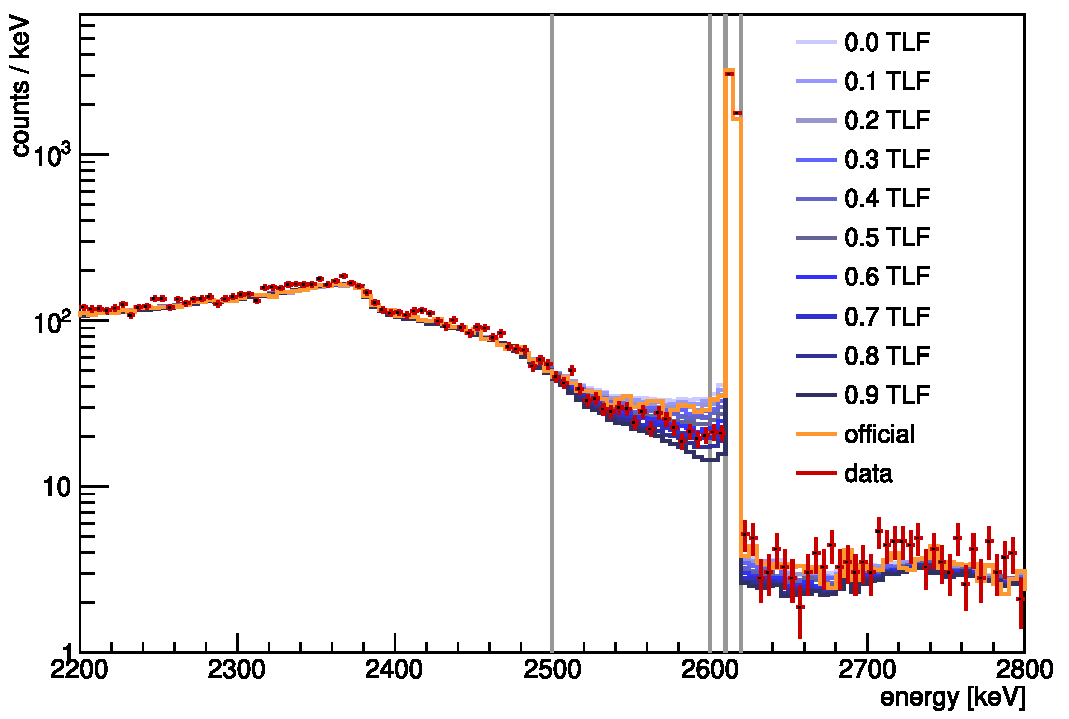
\includegraphics[width=0.5\textwidth]{plots/gedet-av/GD00C-tl-peak.pdf}%
  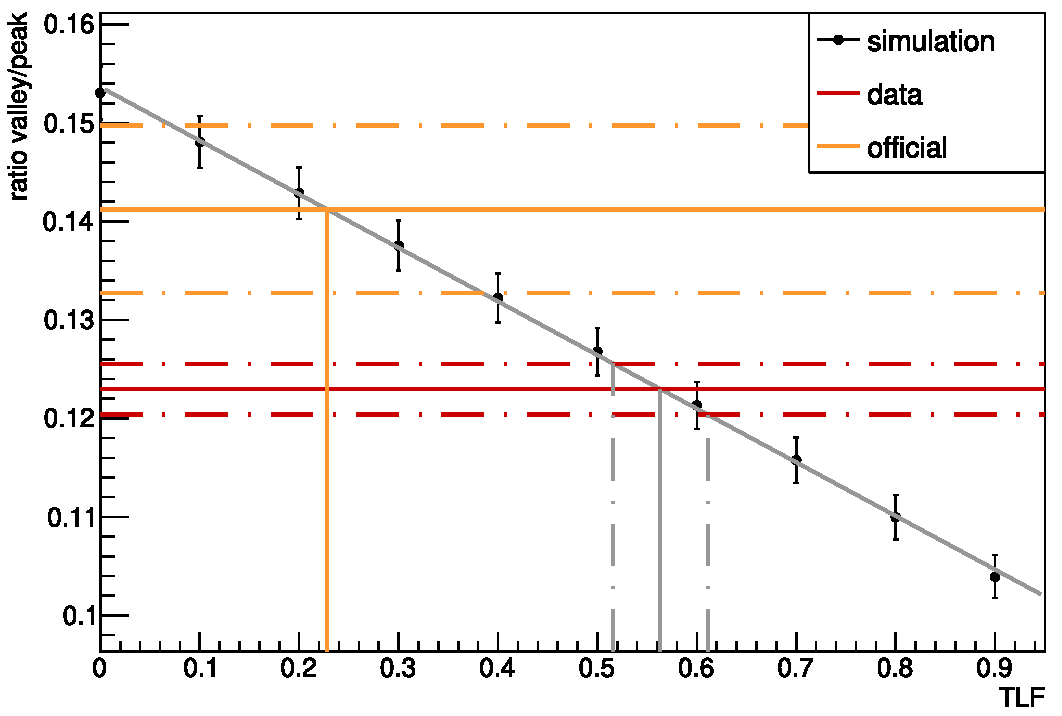
\includegraphics[width=0.5\textwidth]{plots/gedet-av/GD00C-optimization.pdf}
  \caption{%
    Example optimization for detector \GD{00C}. \fillme{update, TLF -> DLF}
  }\label{fig:gedetav:example-optim}
\end{figure}

\section{Insights from \Arl\ data}%
\label{src:gedetav:ar39}

The \gerda\ event spectrum is dominated, at low energies, by \Arl-decay events. This
unstable nucleus is naturally present in the atmosphere and is cosmogenically activated.
It decays to the ground state of $^{39}$K via $\upbeta^-$ decay with a half-life of
269(3)~yr and Q-value of 656(5)~keV. Being commercial liquid argon distilled from air, it
naturally contains a fraction of \Arl, whose activity has been estimated to be of about
1~Bq/kg by various experiments~\cite{Ajaj2019, Calvo2017, Benetti2006, Loosli1983}.
\newpar
The first way a \b\ particle emitted in the \Arl\ decay is detected in \gerda is when it
directly reaches the detector's active volume.

% vim: tw=90
